% Options for packages loaded elsewhere
% Options for packages loaded elsewhere
\PassOptionsToPackage{unicode}{hyperref}
\PassOptionsToPackage{hyphens}{url}
%
\documentclass[
  ignorenonframetext,
  aspectratio=169,
]{beamer}
\newif\ifbibliography
\usepackage{pgfpages}
\setbeamertemplate{caption}[numbered]
\setbeamertemplate{caption label separator}{: }
\setbeamercolor{caption name}{fg=normal text.fg}
\beamertemplatenavigationsymbolsempty
% remove section numbering
\setbeamertemplate{part page}{
  \centering
  \begin{beamercolorbox}[sep=16pt,center]{part title}
    \usebeamerfont{part title}\insertpart\par
  \end{beamercolorbox}
}
\setbeamertemplate{section page}{
  \centering
  \begin{beamercolorbox}[sep=12pt,center]{section title}
    \usebeamerfont{section title}\insertsection\par
  \end{beamercolorbox}
}
\setbeamertemplate{subsection page}{
  \centering
  \begin{beamercolorbox}[sep=8pt,center]{subsection title}
    \usebeamerfont{subsection title}\insertsubsection\par
  \end{beamercolorbox}
}
% Prevent slide breaks in the middle of a paragraph
\widowpenalties 1 10000
\raggedbottom
\AtBeginPart{
  \frame{\partpage}
}
\AtBeginSection{
  \ifbibliography
  \else
    \frame{\sectionpage}
  \fi
}
\AtBeginSubsection{
  \frame{\subsectionpage}
}
\usepackage{iftex}
\ifPDFTeX
  \usepackage[T1]{fontenc}
  \usepackage[utf8]{inputenc}
  \usepackage{textcomp} % provide euro and other symbols
\else % if luatex or xetex
  \usepackage{unicode-math} % this also loads fontspec
  \defaultfontfeatures{Scale=MatchLowercase}
  \defaultfontfeatures[\rmfamily]{Ligatures=TeX,Scale=1}
\fi
\usepackage{lmodern}

\usetheme[]{Madrid}
\usecolortheme[]{default}
\ifPDFTeX\else
  % xetex/luatex font selection
\fi
% Use upquote if available, for straight quotes in verbatim environments
\IfFileExists{upquote.sty}{\usepackage{upquote}}{}
\IfFileExists{microtype.sty}{% use microtype if available
  \usepackage[]{microtype}
  \UseMicrotypeSet[protrusion]{basicmath} % disable protrusion for tt fonts
}{}
\makeatletter
\@ifundefined{KOMAClassName}{% if non-KOMA class
  \IfFileExists{parskip.sty}{%
    \usepackage{parskip}
  }{% else
    \setlength{\parindent}{0pt}
    \setlength{\parskip}{6pt plus 2pt minus 1pt}}
}{% if KOMA class
  \KOMAoptions{parskip=half}}
\makeatother


\usepackage{longtable,booktabs,array}
\usepackage{calc} % for calculating minipage widths
\usepackage{caption}
% Make caption package work with longtable
\makeatletter
\def\fnum@table{\tablename~\thetable}
\makeatother
\usepackage{graphicx}
\makeatletter
\newsavebox\pandoc@box
\newcommand*\pandocbounded[1]{% scales image to fit in text height/width
  \sbox\pandoc@box{#1}%
  \Gscale@div\@tempa{\textheight}{\dimexpr\ht\pandoc@box+\dp\pandoc@box\relax}%
  \Gscale@div\@tempb{\linewidth}{\wd\pandoc@box}%
  \ifdim\@tempb\p@<\@tempa\p@\let\@tempa\@tempb\fi% select the smaller of both
  \ifdim\@tempa\p@<\p@\scalebox{\@tempa}{\usebox\pandoc@box}%
  \else\usebox{\pandoc@box}%
  \fi%
}
% Set default figure placement to htbp
\def\fps@figure{htbp}
\makeatother





\setlength{\emergencystretch}{3em} % prevent overfull lines

\providecommand{\tightlist}{%
  \setlength{\itemsep}{0pt}\setlength{\parskip}{0pt}}



 


\makeatletter
\@ifpackageloaded{caption}{}{\usepackage{caption}}
\AtBeginDocument{%
\ifdefined\contentsname
  \renewcommand*\contentsname{Table of contents}
\else
  \newcommand\contentsname{Table of contents}
\fi
\ifdefined\listfigurename
  \renewcommand*\listfigurename{List of Figures}
\else
  \newcommand\listfigurename{List of Figures}
\fi
\ifdefined\listtablename
  \renewcommand*\listtablename{List of Tables}
\else
  \newcommand\listtablename{List of Tables}
\fi
\ifdefined\figurename
  \renewcommand*\figurename{Figure}
\else
  \newcommand\figurename{Figure}
\fi
\ifdefined\tablename
  \renewcommand*\tablename{Table}
\else
  \newcommand\tablename{Table}
\fi
}
\@ifpackageloaded{float}{}{\usepackage{float}}
\floatstyle{ruled}
\@ifundefined{c@chapter}{\newfloat{codelisting}{h}{lop}}{\newfloat{codelisting}{h}{lop}[chapter]}
\floatname{codelisting}{Listing}
\newcommand*\listoflistings{\listof{codelisting}{List of Listings}}
\makeatother
\makeatletter
\makeatother
\makeatletter
\@ifpackageloaded{caption}{}{\usepackage{caption}}
\@ifpackageloaded{subcaption}{}{\usepackage{subcaption}}
\makeatother

\usepackage{bookmark}
\IfFileExists{xurl.sty}{\usepackage{xurl}}{} % add URL line breaks if available
\urlstyle{same}
\hypersetup{
  pdftitle={Model-assisted estimation for forest inventories},
  pdfauthor={Alexander Massey},
  hidelinks,
  pdfcreator={LaTeX via pandoc}}


\title{Model-assisted estimation for forest inventories}
\subtitle{A Monte Carlo approach}
\author{Alexander Massey}
\date{2026-09-11}

\begin{document}
\frame{\titlepage}


\begin{frame}{Sample unit is a point}
\phantomsection\label{sample-unit-is-a-point}
\begin{columns}[T]
\begin{column}{0.58\linewidth}
\begin{center}
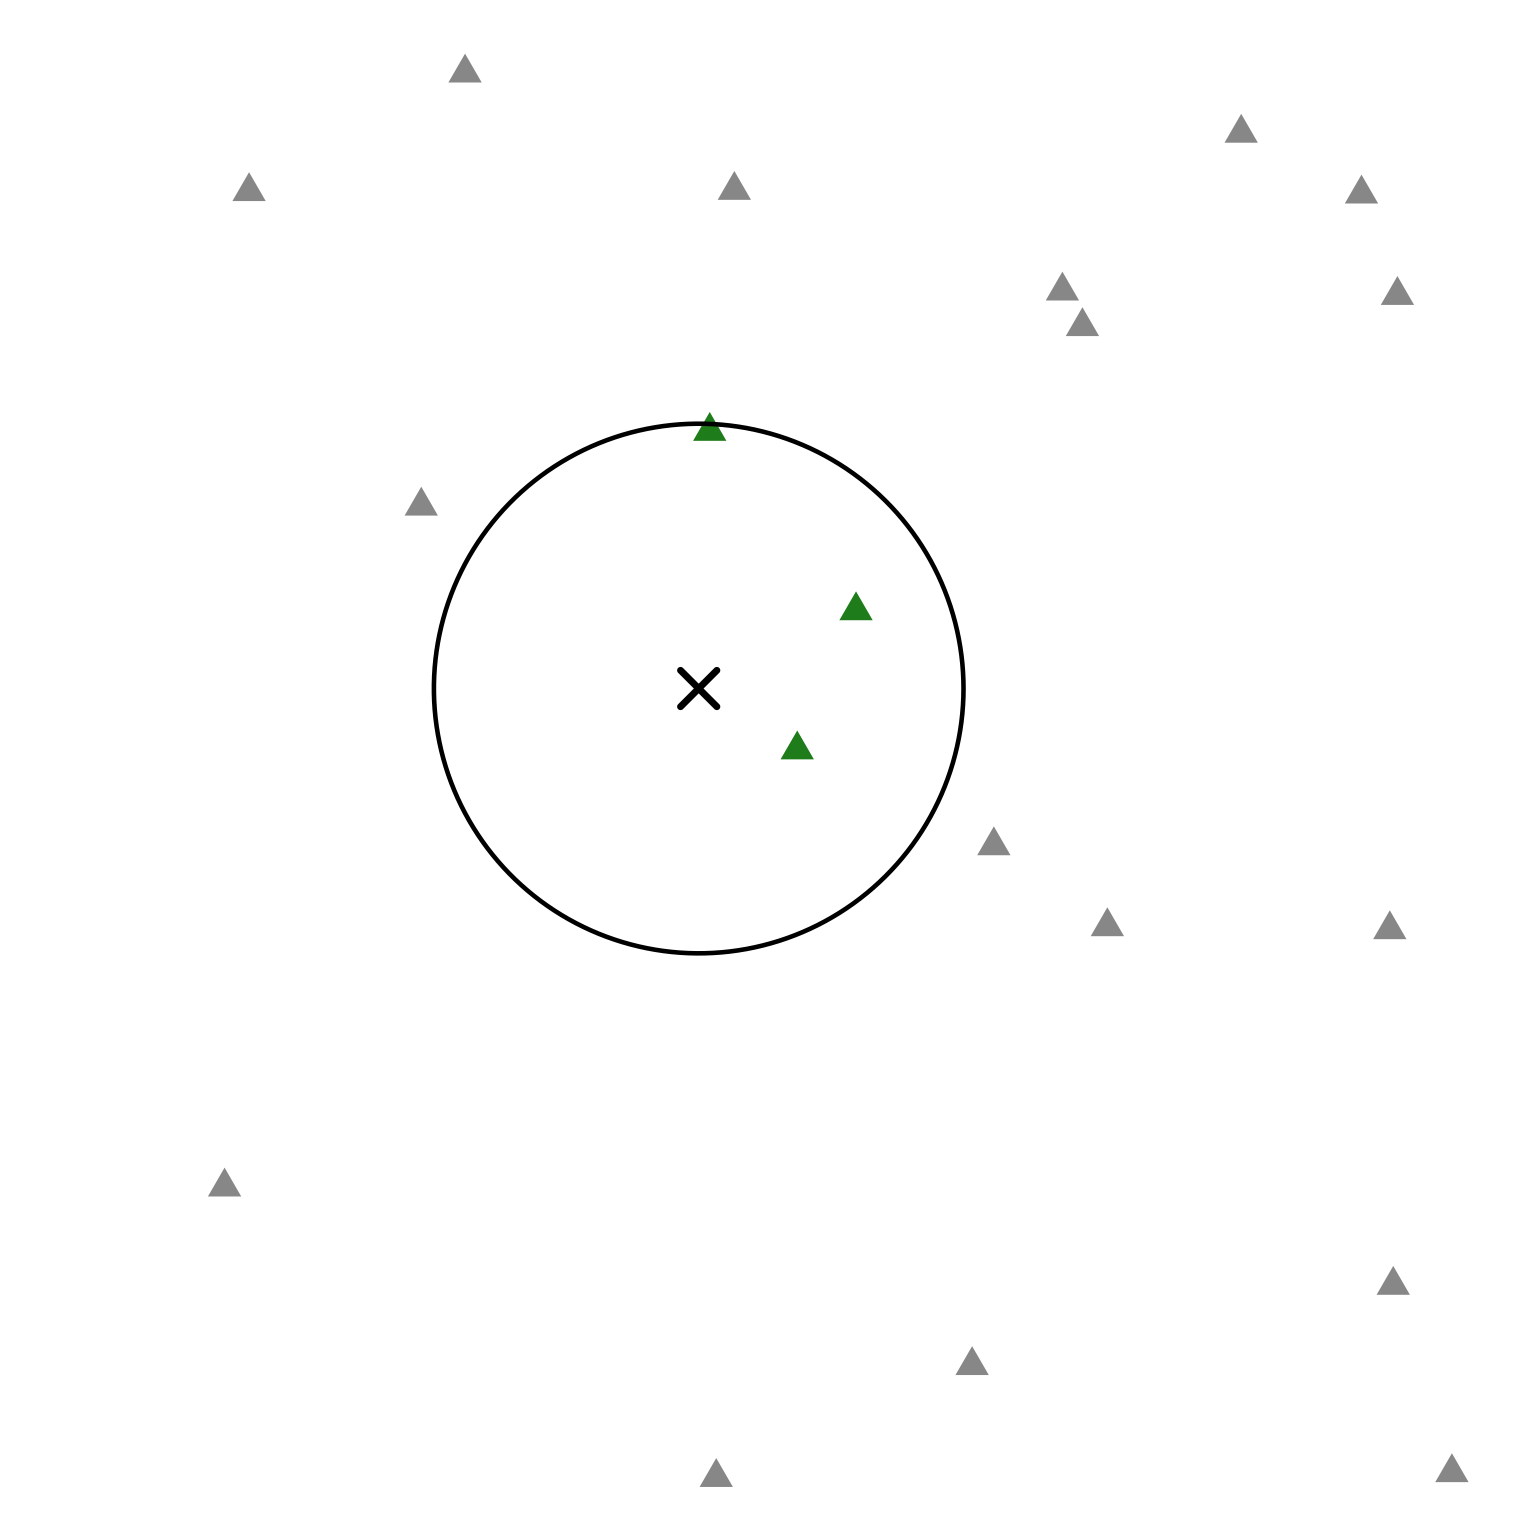
\includegraphics[width=1\linewidth,height=\textheight,keepaspectratio]{monte_carlo_interpretation_beamer_files/figure-beamer/unnamed-chunk-2-1.png}
\end{center}
\end{column}

\begin{column}{0.42\linewidth}
\footnotesize
\begin{itemize}
    \item A circular plot is centered on the \textbf{sample point} selects trees inside the inclusion radius.
    \item[] 
    \item Multiple inclusion radii are possible based on DBH thresholds.
    \item[]
    \item There are infinite points in the forest.
    \item[]
    \item \textbf{Finite population sampling theory} is commonly used but the problem is poorly posed.
    \item[]
    \item Circles do not tesselate! Angle count sampling makes no sense...
\end{itemize}
\end{column}
\end{columns}
\end{frame}

\begin{frame}{\textbf{Workaround:} Draw same inclusion rings around
trees}
\phantomsection\label{draw-same-inclusion-rings-around-trees}
\begin{columns}[T]
\begin{column}{0.58\linewidth}
\begin{center}
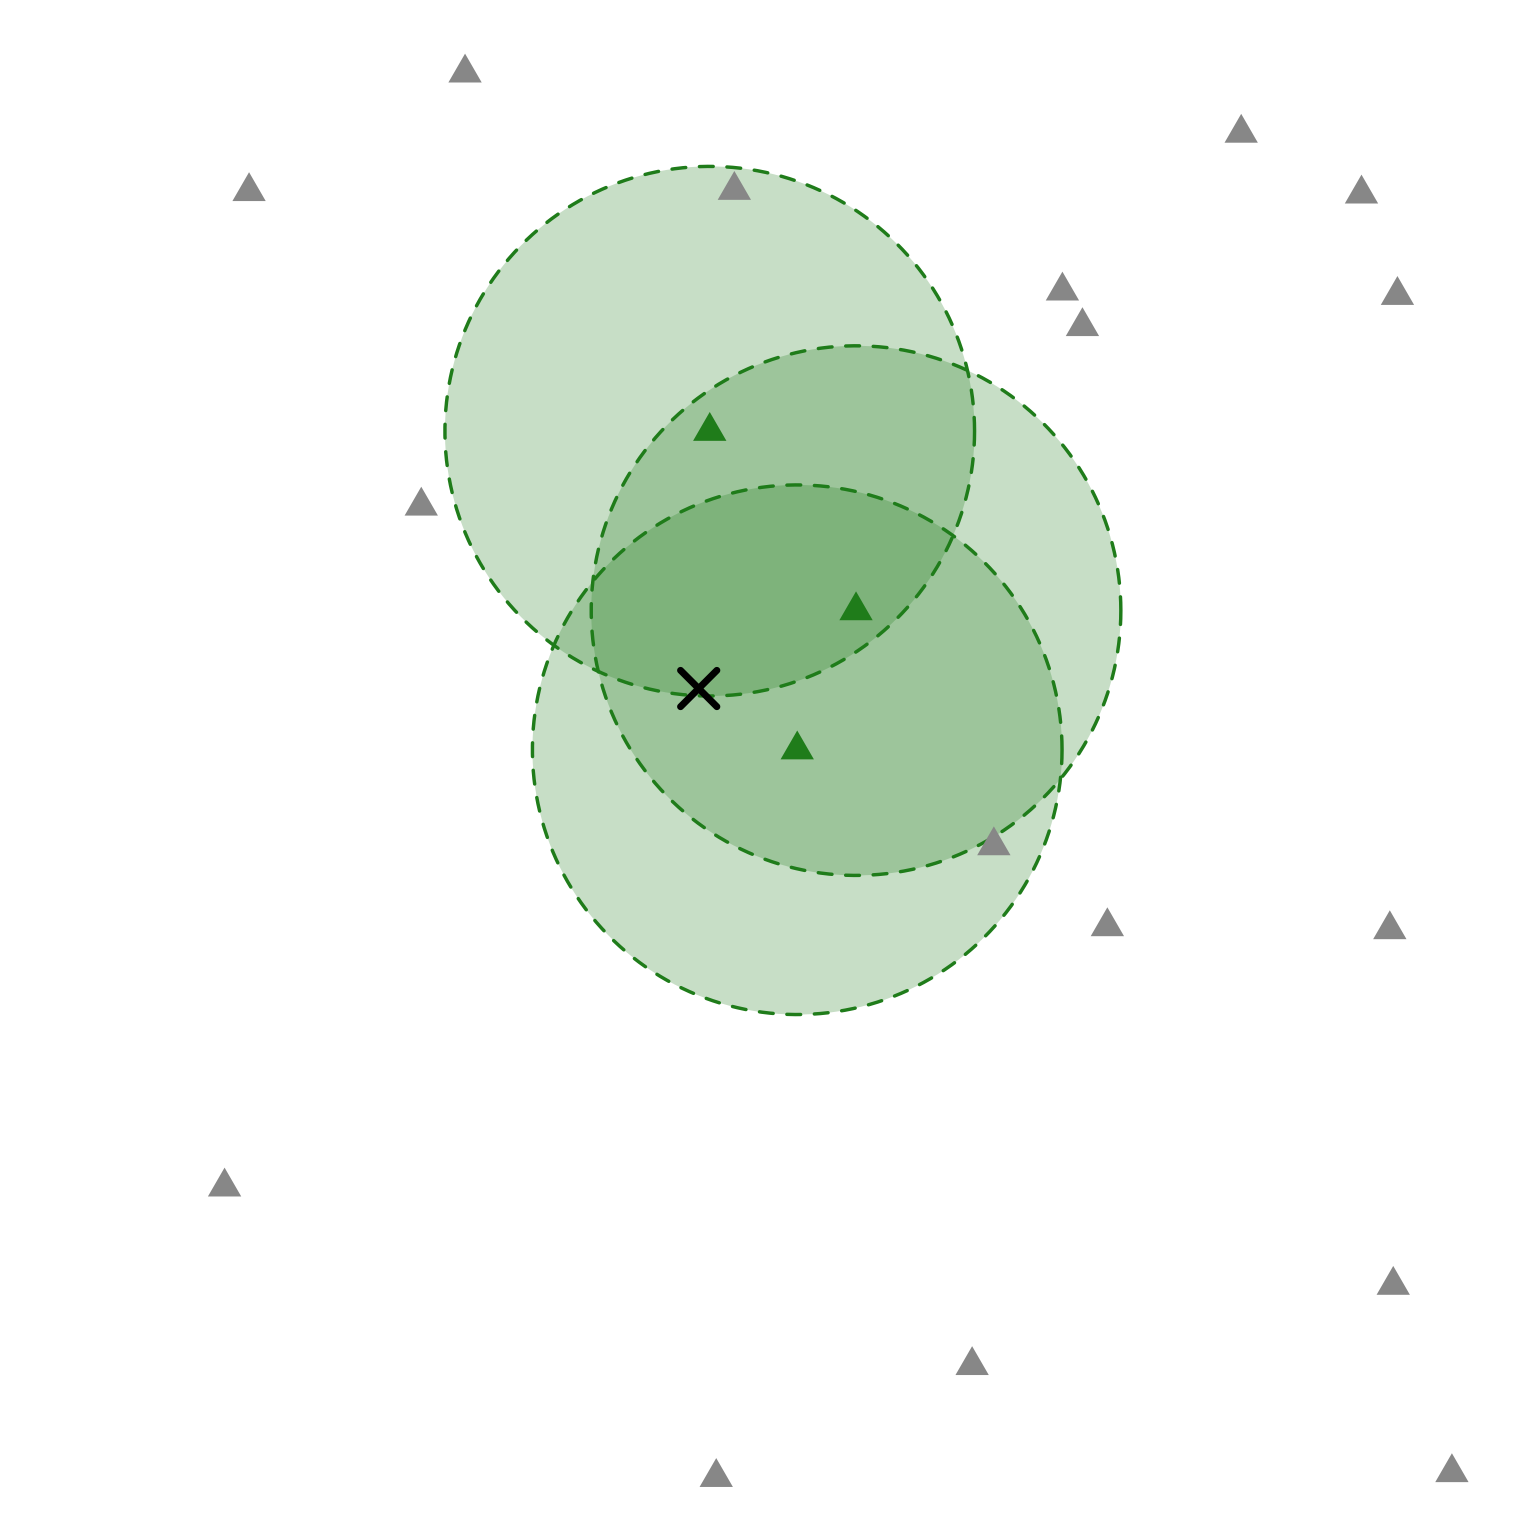
\includegraphics[width=1\linewidth,height=\textheight,keepaspectratio]{monte_carlo_interpretation_beamer_files/figure-beamer/unnamed-chunk-3-1.png}
\end{center}
\end{column}

\begin{column}{0.42\linewidth}
\footnotesize
\begin{definition}[Duality principle]
trees in radius around point same as point in radius around trees.
\end{definition}
\begin{itemize}
    \item[]
    \item Overlap of the inclusion rings illustrates density accumulation at a point.
    \item[]
    \item Sample unit is the point; not the trees.
    \item[]
\end{itemize}

\begin{description}
\tightlist
\item[\(x\)]
point at plot center
\end{description}
\end{column}
\end{columns}
\end{frame}

\begin{frame}{Boundary adjustment on trees (not plots)}
\phantomsection\label{boundary-adjustment-on-trees-not-plots}
\begin{columns}[T]
\begin{column}{0.58\linewidth}
\begin{center}
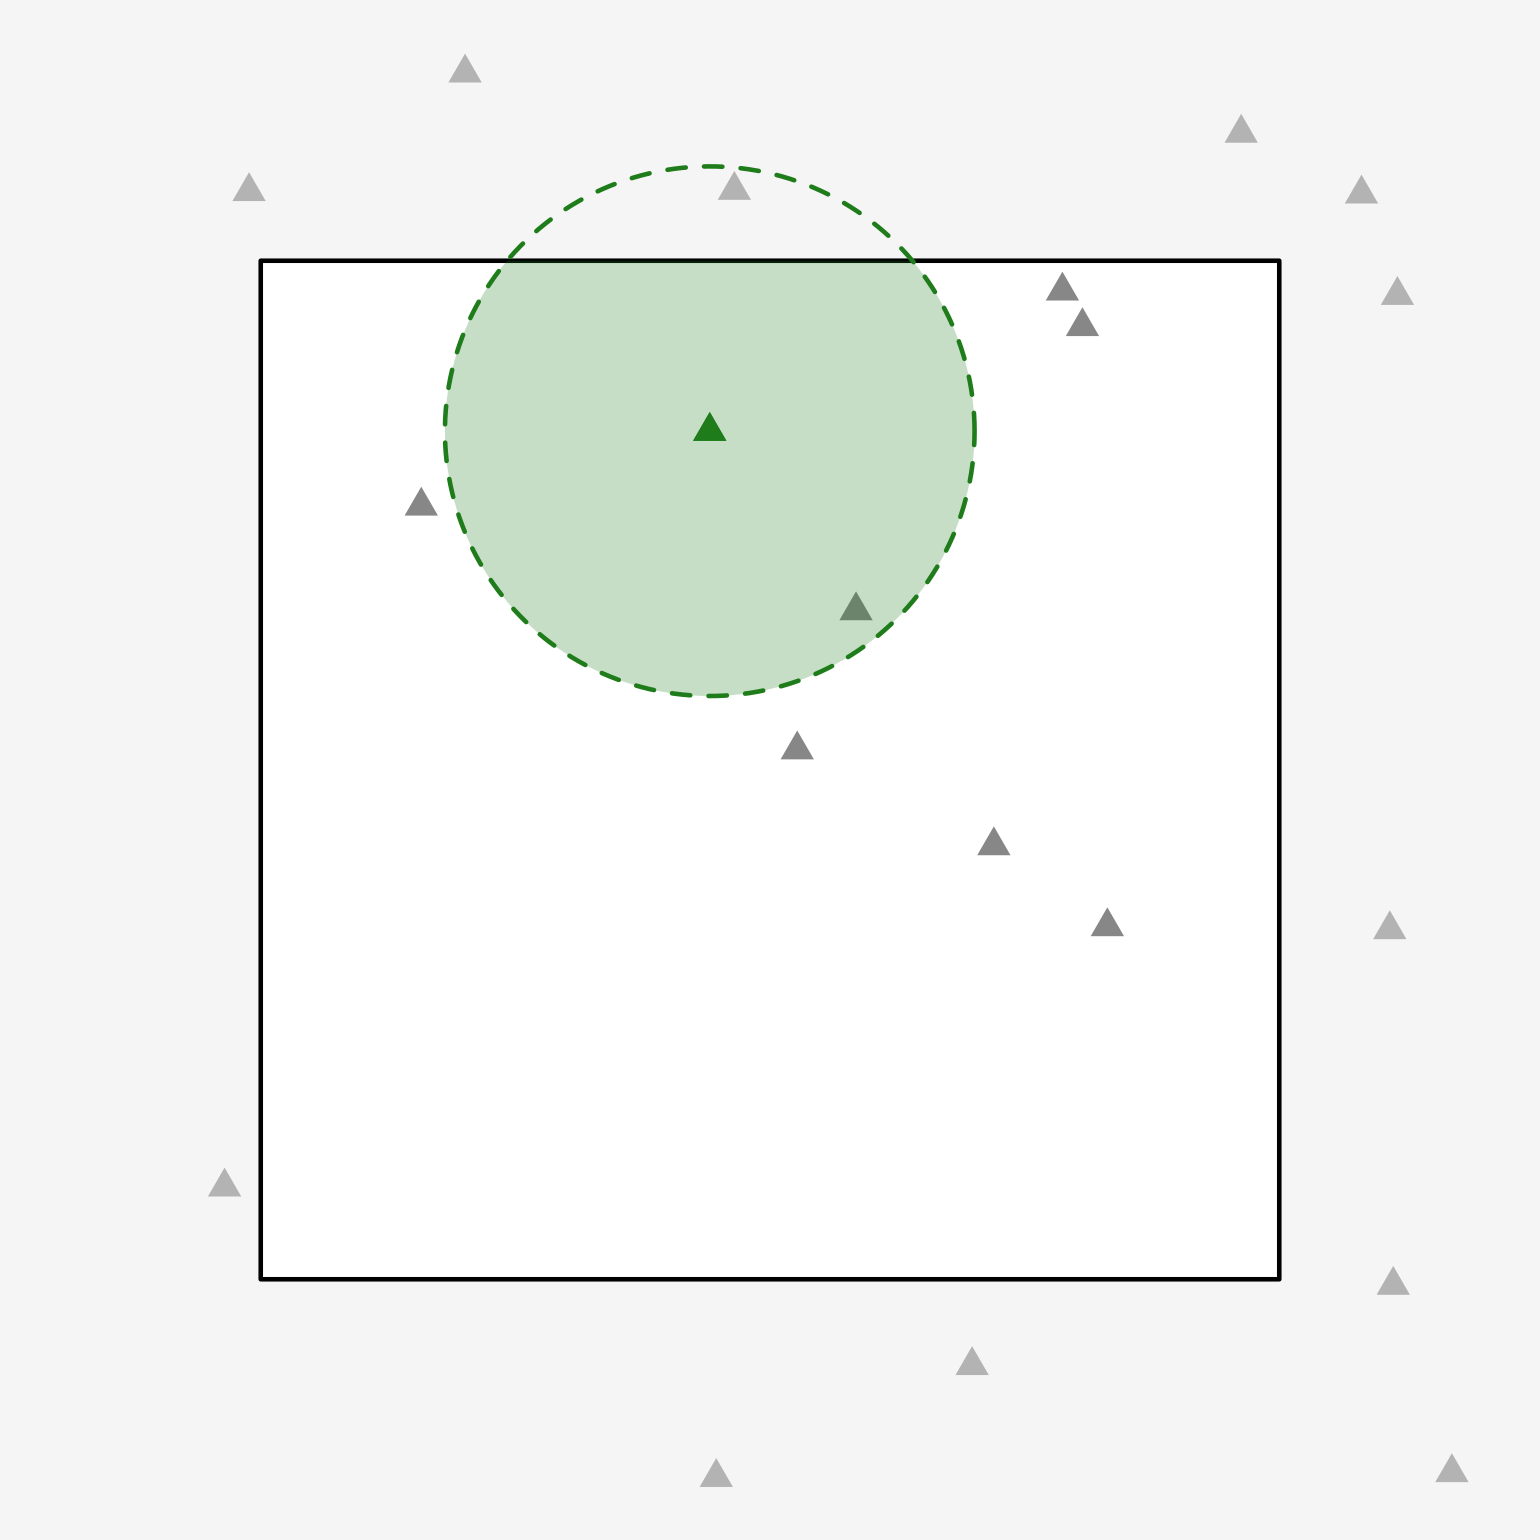
\includegraphics[width=1\linewidth,height=\textheight,keepaspectratio]{monte_carlo_interpretation_beamer_files/figure-beamer/unnamed-chunk-4-1.png}
\end{center}
\end{column}

\begin{column}{0.42\linewidth}
\footnotesize

\begin{itemize}
\item
  Plots with centers outside forest (gray) are \textbf{not visited} for
  budget reasons.
\item
  Requires boundary adjustment for \textbf{trees}.
\end{itemize}

\begin{definition}[Indicator variable]
\[
  I_i(x)=
  \begin{cases}
  1,&\text{if }x\in K_i,\\
  0,&\text{if }x\notin K_i.
  \end{cases}
\]
\end{definition}

\begin{definition}[Inclusion probability]
\[
  \pi_i = \mathbb{P}[I_i(x)] = \mathbb{E}[I_i(x)] =
  \frac{A_{K_i}}{A_T}
\]
\end{definition}

\begin{description}
\tightlist
\item[\(K_i\)]
inclusion ring around tree \(i\)
\item[\(A_T\) ; \(A_{K_i}\)]
area of \(T\) ; \(K_i\) (bnd. adjusted)
\item[\(T\)]
territory of interest
\end{description}
\end{column}
\end{columns}
\end{frame}

\begin{frame}{Local density surface from above}
\phantomsection\label{local-density-surface-from-above}
\begin{columns}[T]
\begin{column}{0.58\linewidth}
\begin{center}
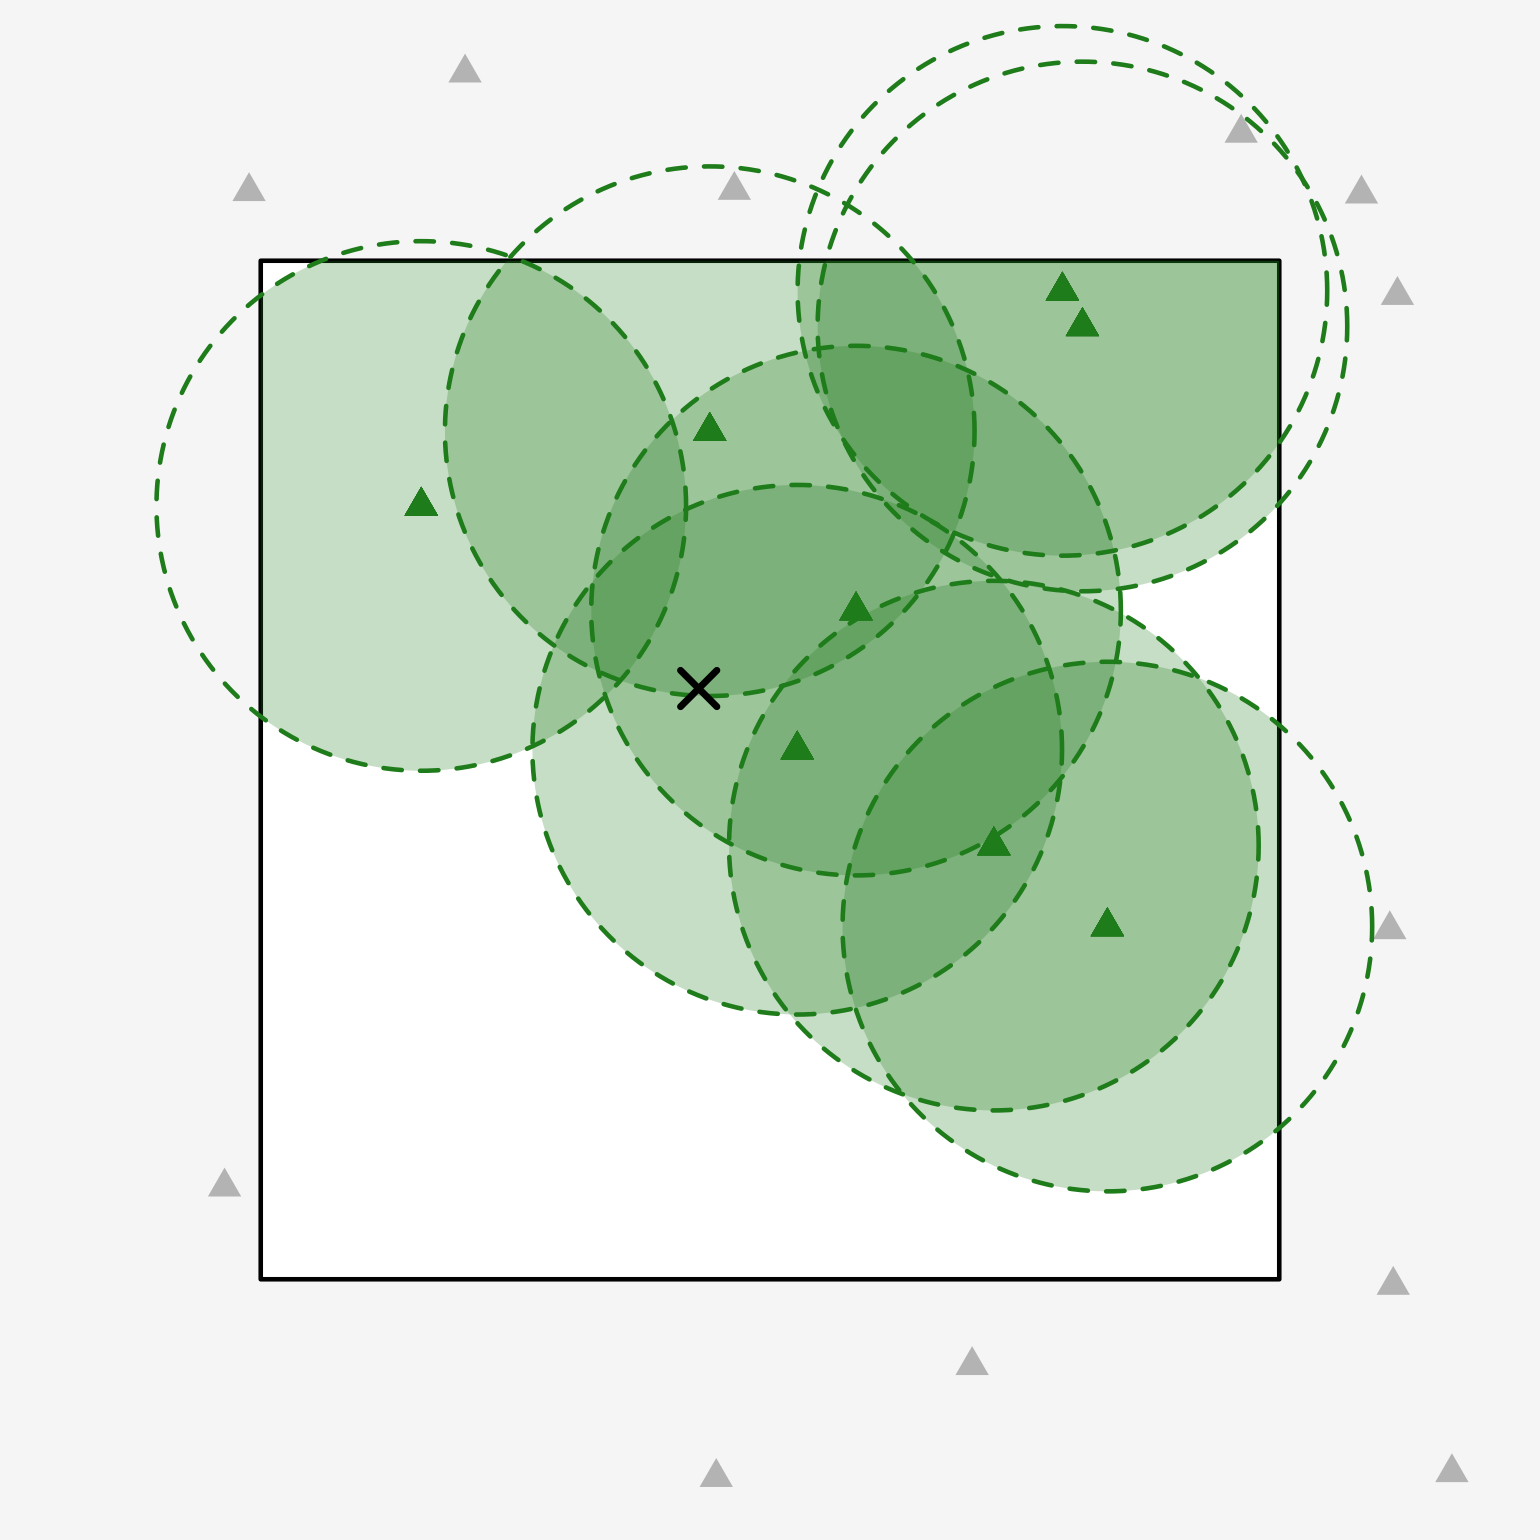
\includegraphics[width=1\linewidth,height=\textheight,keepaspectratio]{monte_carlo_interpretation_beamer_files/figure-beamer/unnamed-chunk-5-1.png}
\end{center}
\end{column}

\begin{column}{0.42\linewidth}
\footnotesize
\centering

\textbf{\underline{Surface is fixed; point is random}}

\begin{definition}[Local density surface]

\[
Y(x)=\frac{1}{A_T}\sum_{i=1}^N\frac{I_i(x)Y_i}{\pi_i}
\]

\end{definition}

\begin{description}
\tightlist
\item[\(Y_i\)]
measurement for tree \(i\)
\item[\(\pi_i\)]
inclusion probability for tree \(i\)
\item[\(N\)]
number of trees in territory \(T\)
\item[\(I_i(x)\)]
indicator that tree \(i\) is selected at \(x\)
\item[\(A_T\)]
surface area of \(T\)
\end{description}

\begin{block}{Interpretation}

$Y(x)$ is the Horvitz--Thompson estimator (for the spatial) mean with sample size one.

\end{block}
\end{column}
\end{columns}
\end{frame}

\begin{frame}{Monte Carlo integration --- a reminder}
\phantomsection\label{monte-carlo-integration-a-reminder}
\begin{columns}[T]
\begin{column}{0.6\linewidth}
\vspace{0cm}

\begin{center}
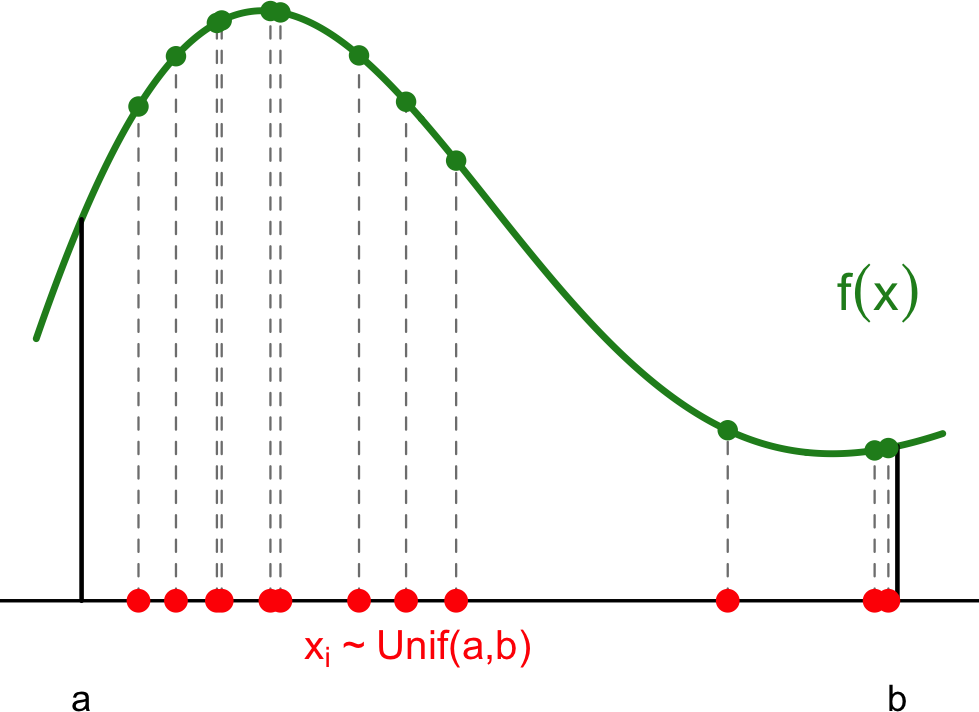
\includegraphics[width=1\linewidth,height=\textheight,keepaspectratio]{monte_carlo_interpretation_beamer_files/figure-beamer/unnamed-chunk-6-1.png}
\end{center}
\end{column}

\begin{column}{0.4\linewidth}
\vspace{0.6cm}
\footnotesize

\textbf{Steps}

\begin{enumerate}
\setlength{\itemsep}{4pt}
\item Draw $x_1,\dots,x_n$ uniform \& independent on $[a,b]$
\item Evaluate $f(x_i)$
\item Average: $\bar f = \frac{1}{n}\sum_i f(x_i)$
\item Scale by domain length:
\[
\int_a^b f(x)\,dx \approx (b-a)\bar f
\]
\end{enumerate}
\vspace{4pt}
\footnotesize

\textbf{Law of Large Numbers} \newline \(\bar f \to \mathbb{E}[f(x)]\))
\newline\newline \textbf{Central Limit Theorem}
\newline \(\sqrt{n}(\bar f - \mathbb{E}[f(x)]) \xrightarrow{d} \mathcal{N}(0,\sigma^2)\)
\textcolor{gray}{(for CIs)}
\end{column}
\end{columns}
\end{frame}

\begin{frame}{Exercise --- Prove equivalence of sampling trees and Monte
Carlo integration}
\phantomsection\label{exercise-prove-equivalence-of-sampling-trees-and-monte-carlo-integration}
\footnotesize
\centering
\begin{block}{Show (assume uniform independent sampling)}
\[
A_T \cdot \mathbb{E}[Y(x)] \;=\; \int_T Y(x)\,dx \;=\; \sum_{i=1}^{N} Y_i
\]
\vspace{0.25em}
\flushright \textcolor{gray}{\textbf{Hint :}  $\mathbb{E}[g(X)] = \int g(x)\,f(x)\,dx
\qquad\text{and}\qquad
\mathbb{E}[I_i(x)] = \pi_i$}
\end{block}
\pause
\begin{proof}
\begin{align}
\onslide<2->{A_T \cdot \mathbb{E}[Y(x)]
  &= A_T \cdot \int_T Y(x)\,\underbrace{\frac{1}{A_T}}_{f(x)}\,dx
   =\int_T Y(x)\,dx} \\
\onslide<3->{A_T \cdot \mathbb{E}[Y(x)]
  &=  A_T \cdot \mathbb{E}\!\left[\frac{1}{A_T}\sum_{i=1}^N \frac{I_i(x)\,Y_i}{\pi_i}\right]
   = \sum_{i=1}^N \frac{Y_i}{\pi_i}\,\mathbb{E}[I_i(x)] = \sum_{i=1}^N \frac{Y_i}{\pi_i}\cdot \pi_i
   = \sum_{i=1}^N Y_i}
\end{align}
\end{proof}
\end{frame}

\begin{frame}{View of 3d local density surface from artificial forest}
\phantomsection\label{view-of-3d-local-density-surface-from-artificial-forest}
Not so useful\ldots{} It is easier to simplify the dimension. \centering
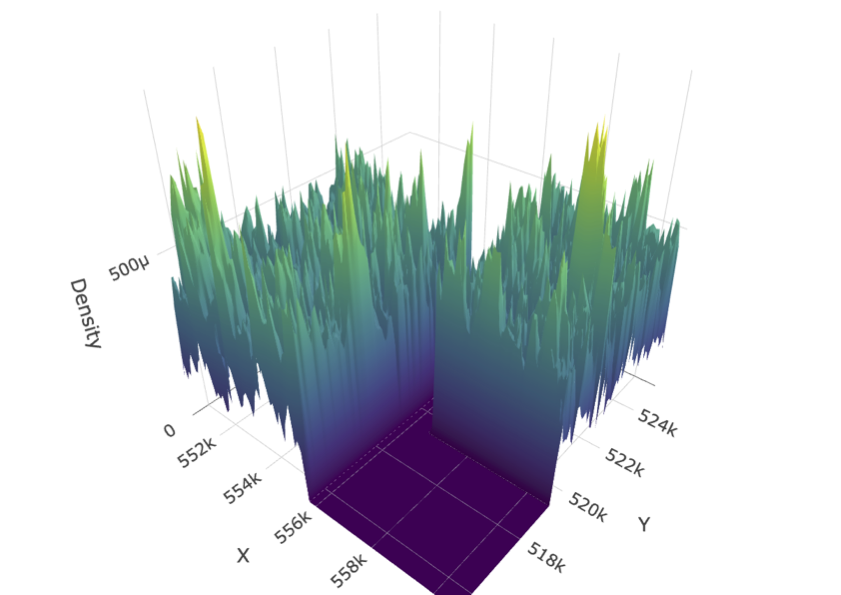
\includegraphics[width=0.6\linewidth,height=\textheight,keepaspectratio]{images/simulation_surface.png}
\end{frame}

\begin{frame}{Heuristic representation of Monte Carlo approach}
\phantomsection\label{heuristic-representation-of-monte-carlo-approach}
\centering
\only<1>{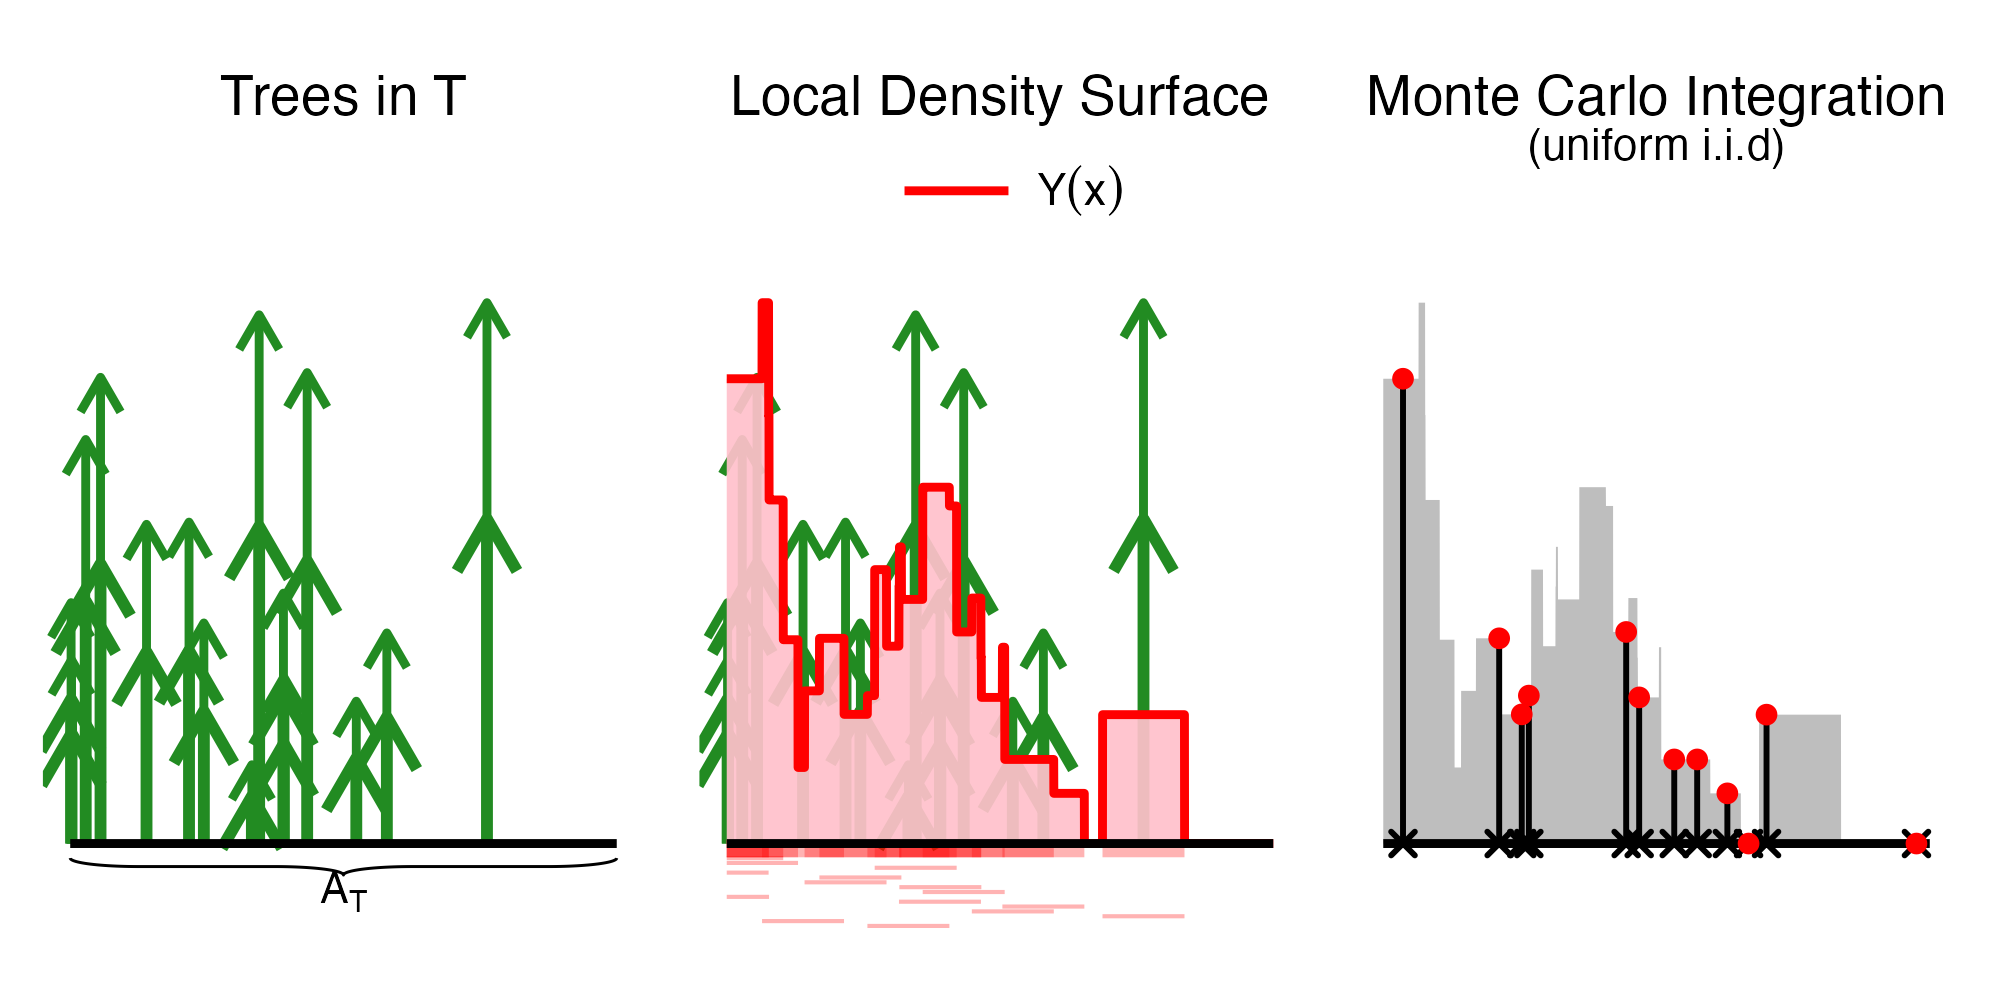
\includegraphics[width=\textwidth]{fig_build1.png}}
\only<2>{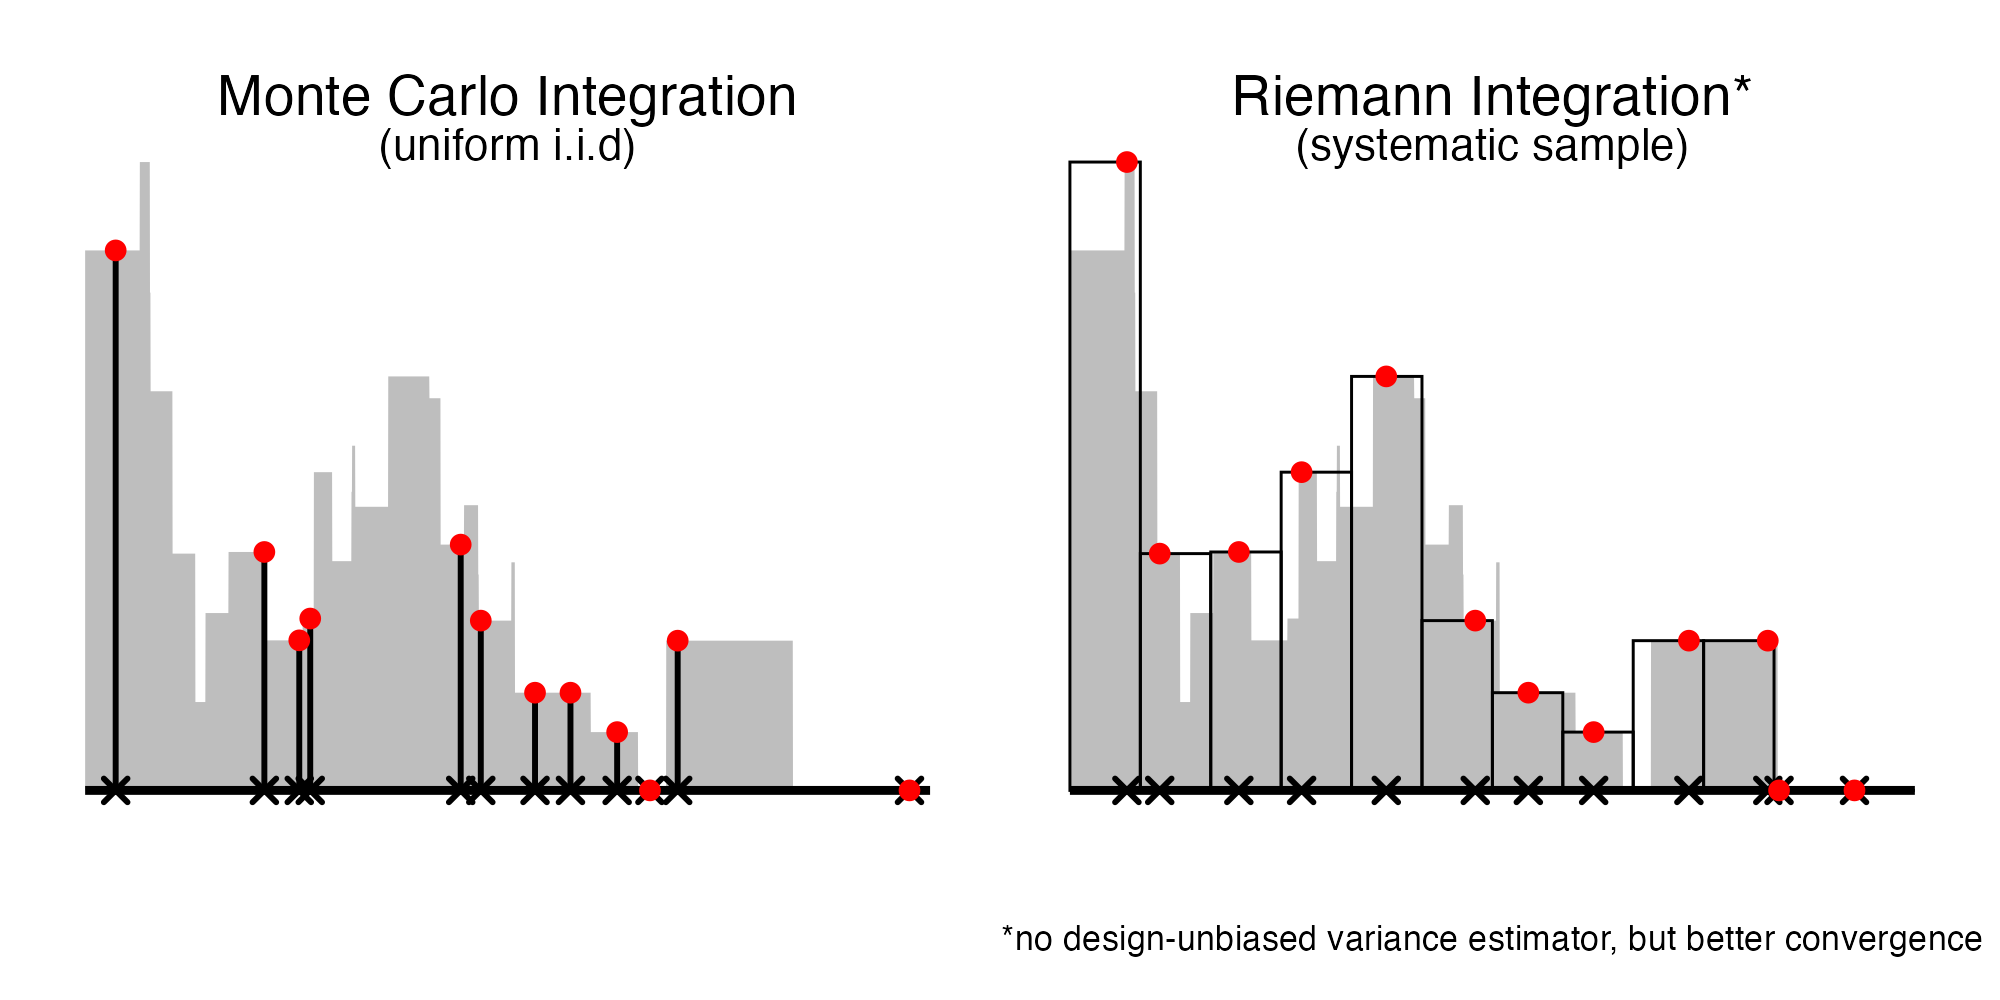
\includegraphics[width=\textwidth]{fig_build2.png}}
\end{frame}

\begin{frame}{One-phase estimation for uniform independent sampling}
\phantomsection\label{one-phase-estimation-for-uniform-independent-sampling}
\footnotesize
\centering

\begin{block}{Population parameters and their sample-copy estimators}
Assume $A_T$ is known.
\vspace{4pt}

\begin{tabular}{l r c l @{\hspace{3em}} r c l}
\textbf{Population} &
  $\mathbb{E}[Y(x)]$ & $=$ & $\dfrac{1}{A_T}\displaystyle\int_T Y(x)\,dx$ &
  $\mathbb{V}[Y(x)]$ & $=$ & $\dfrac{1}{A_T}\displaystyle\int_T \big(Y(x)-\mathbb{E}[Y(x)]\big)^2 dx$ \\[10pt]
\textbf{\textit{"Sample copy"}} &
  $\bar Y_s$ & $=$ & $\dfrac{1}{n}\displaystyle\sum_{x \in s} Y(x)$ &
  $\hat{\mathbb{V}}[Y(x)]$ & $=$ & $\dfrac{1}{n-1}\displaystyle\sum_{x \in s}\big(Y(x)-\bar Y_s\big)^2$ \\
\end{tabular}
\end{block}

\pause

\begin{definition}[One-phase point and variance estimator]
Draw $x \in s$, $n$ times, uniformly and independently.
\vspace{4pt}

\[
\hat Y_{1p} \;=\; \frac{1}{n}\sum_{x \in s} Y(x)
\quad\quad\quad
\mathbb{V}[\hat Y_{1p}]=\frac{\mathbb{V}[Y(x)]}{n}
\quad\quad\quad
\hat{\mathbb{V}}[\hat Y_{1p}]=\frac{\hat{\mathbb{V}}[Y(x)]}{n}
\]
\end{definition}

Every point estimator has a population variance estimated by a (sample)
variance estimator.
\end{frame}

\begin{frame}{Short view of the classical survey sampling theory (Cordy,
1993)}
\phantomsection\label{short-view-of-the-classical-survey-sampling-theory-cordy-1993}
\footnotesize

\begin{itemize}
\tightlist
\item
  For fixed sample size \(n\), denote the sample
  \(s = \{x_1, x_2, \dots, x_n\} \subset T\).
\item
  Under \textbf{uniform i.i.d.} sampling, every \(x_k\) has the same
  marginal density \(f(x) = 1/A_T\).
\item
  The \textbf{sampling intensity} (inclusion prob. from finite theory)
  is \[
  \pi(x) = \sum_{k=1}^n f(x) = n\,f(x) = \frac{n}{A_T}, \qquad x \in T
  \]
\item
  The \textbf{second-order sampling intensity} (probability of a pair
  being jointly sampled) is \[
  \pi(x,x') = \sum_{k=1}^n\sum_{j\neq k} f(x)f(x') = n(n-1)\,f(x)f(x') = \frac{n(n-1)}{A_T^2}, \qquad x \neq x'
  \]
\end{itemize}

\pause

\begin{block}{Note}
General survey sampling allows $f_k(x)$ to vary by draw or be non-uniform (importance sampling, unequal probability designs). Under uniform i.i.d.\ sampling both intensities collapse to constants --- they don't depend on $x$ at all.
\end{block}
\end{frame}

\begin{frame}{Horvitz--Thompson estimator and Yates--Grundy variance}
\phantomsection\label{horvitzthompson-estimator-and-yatesgrundy-variance}
\footnotesize

\begin{block}{General form}
\[
\hat Y = \sum_{x \in s} w(x)\,Y(x)
\]
The \textbf{Horvitz--Thompson estimator} sets $w(x) = 1/\pi(x)$ and is design-unbiased whenever $\pi(x) > 0$ for all $x \in T$.
\end{block}

\pause

\begin{block}{Yates--Grundy variance estimator}
Unbiased under regularity conditions (most notably fixed $n$ and $\pi(x,x') > 0$):
\[
\hat{\mathbb{V}}(\hat Y_\pi) = -\frac{1}{2}\sum_{x \in s}\sum_{x' \neq x} \frac{\pi(x,x') - \pi(x)\pi(x')}{\pi(x,x')} \left(\frac{Y(x)}{\pi(x)} - \frac{Y(x')}{\pi(x')}\right)^2
\]
\end{block}
\end{frame}

\begin{frame}{Several minutes later\ldots{}}
\phantomsection\label{several-minutes-later}
\begin{block}{Plug in uniform i.i.d.\ intensities}
With $\pi(x) = n/A_T$ and $\pi(x,x') = n(n-1)/A_T^2$, tedious algebra recovers exactly what we already had from Monte Carlo integration:
\[
\hat Y_\pi = A_T \cdot \hat Y_{1p} = A_T \cdot \frac{1}{n}\sum_{x \in s} Y(x)
\qquad\qquad
\hat{\mathbb{V}}(\hat Y_\pi) = \hat{\mathbb{V}}[\hat Y_{1p}] = \frac{\hat{\mathbb{V}}[Y(x)]}{n}
\]
\end{block}

\pause

\begin{block}{Why bother?}
This is how most people construct their understanding for forest inventory sampling (although usually for finite population theory). 

---

The \textbf{Monte Carlo approach} lets you more easily visualize, build intuition and derive a surprising number of valuable estimators.
\end{block}
\end{frame}

\begin{frame}{Model-assisted estimation under the Monte Carlo approach}
\phantomsection\label{model-assisted-estimation-under-the-monte-carlo-approach}
\begin{center}
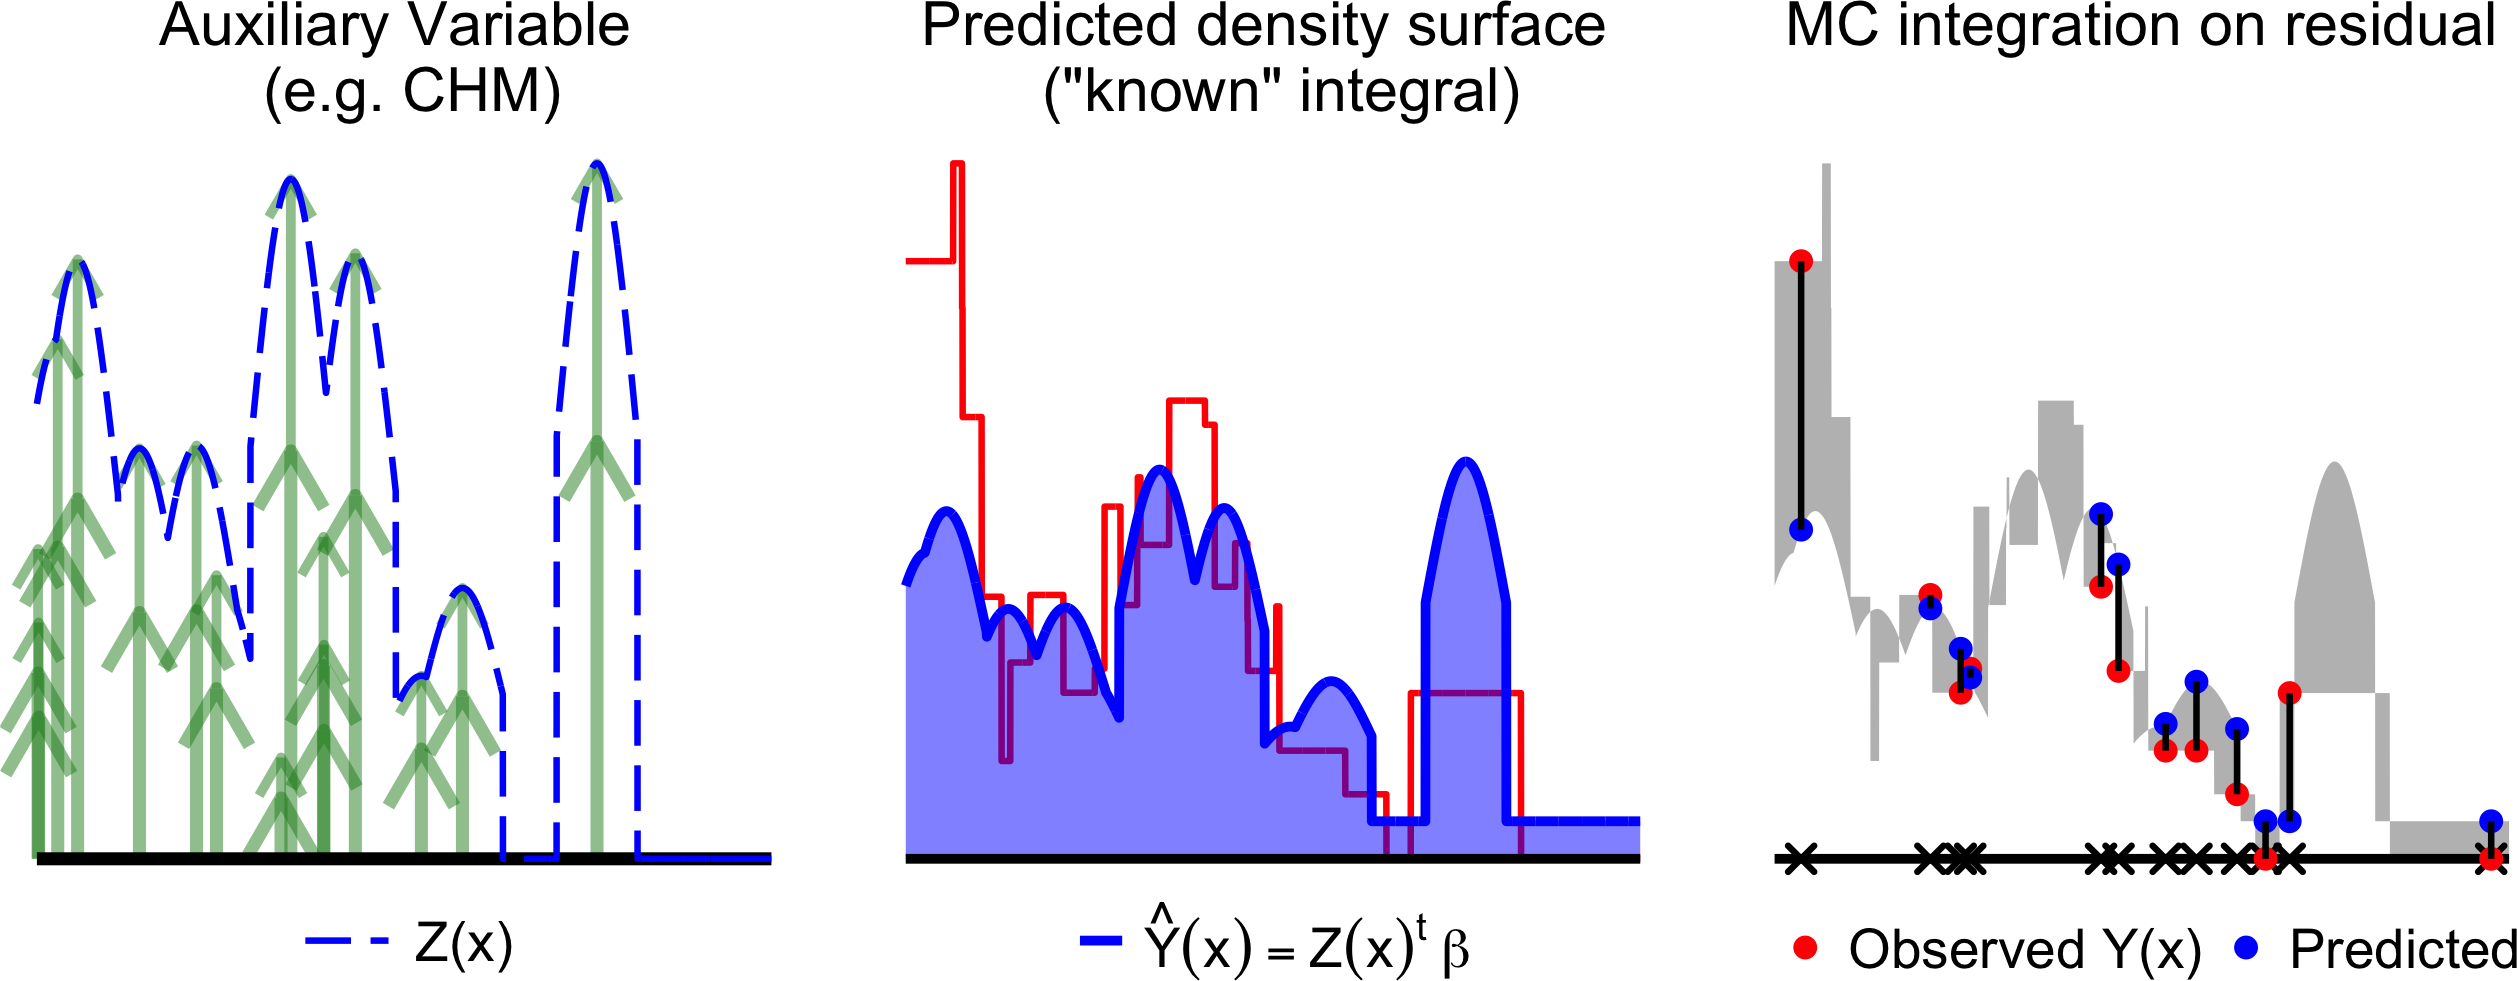
\includegraphics[width=1\linewidth,height=\textheight,keepaspectratio]{monte_carlo_interpretation_beamer_files/figure-beamer/unnamed-chunk-8-1.png}
\end{center}
\end{frame}

\begin{frame}{The difference estimator}
\phantomsection\label{the-difference-estimator}
\begingroup
\renewcommand{\arraystretch}{1.6}
\begin{tabular}{@{}p{0.30\textwidth} r c l@{}}
\textcolor{blue}{\textbf{Sampling design}} &
  \multicolumn{3}{l}{Uniform iid sampling} \\[1.5em]

\textcolor{blue}{\textbf{Point estimator}} &
  $\hat{Y}_{diff}$ & $=$ &
  $\displaystyle \frac{1}{A_T} \int_{T} \hat{Y}(x)\, dx + \frac{1}{n} \sum_{x \in s} R(x)$ \\[1.5em]

\textcolor{blue}{\textbf{Population variance}} &
  $\mathbb{V}[\hat{Y}_{diff}]$ & $=$ &
  $\displaystyle \mathbb{V}\left[\frac{1}{A_T} \int_{T} \hat{Y}(x)\, dx + \frac{1}{n} \sum_{x \in s} R(x)\right]$ \\
 & & $=$ &
  $\displaystyle \frac{1}{n} \mathbb{V}[R(x)]$ \\[1.5em]

\textcolor{blue}{\textbf{Variance estimator}} &
  $\hat{\mathbb{V}}[\hat{Y}_{diff}]$ & $=$ &
  $\displaystyle \frac{1}{n} \hat{\mathbb{V}}_{s}[R(x)]$ \\
\end{tabular}
\endgroup
\end{frame}

\begin{frame}{\textbf{Example}: ``Model-assisted'' using plug-in
estimation:}
\phantomsection\label{model-assisted-using-plug-in-estimation}
\[
\begin{array}{c @{\hspace{2cm}} l}
\begin{aligned}
Y(x):= \mathbf{Z}(x)^t\boldsymbol{\beta} + R(x)
\end{aligned}
& \text{\textcolor{blue}{\textit{"assisting model"} proposal}} \\[10pt]
\begin{aligned}
\hat{Y}(x) = \mathbf{Z}(x)^t\boldsymbol{\hat\beta}
\hspace{1.5cm}
\hat{R}(x) = Y(x) - \hat{Y}(x)
\end{aligned}
& \text{\textcolor{blue}{\textit{Plug-ins}}}
\end{array}
\]

\begin{itemize}
\item[-] $\hat{\boldsymbol{\beta}}$ fit independently of $s$ (i.e. external) $\implies$ exactly design-unbiased.
\item[-] $\hat{\boldsymbol{\beta}}$ fit includes $s$ (i.e. internal) $\implies$ asy. design-unbiased (for "most" choices of $\hat{\boldsymbol{\beta}}$).
\begin{itemize}
\item[] \textcolor{gray}{Note: better variance estimators likely exist (g-weight, bootstrap, etc)}
\end{itemize}
\end{itemize}
\end{frame}

\begin{frame}{External models}
\phantomsection\label{external-models}
\footnotesize

\begin{definition}[External model]
An assisting model $\hat{Y}(x) = \hat m(x)$ is \textbf{external} if the training set used to fit it is independent of the sample $s$ in target territory $T$.
\end{definition}

\pause

\begin{itemize}
\tightlist
\item
  If the model is external, the \(\hat{\bar{Y}}_{diff}\) and variance
  estimator are \textbf{exactly design-unbiased}.
\item
  This holds for \textbf{any} model class \(\hat m(\cdot)\) ---
  parametric or not:

  \begin{itemize}
  \tightlist
  \item
    Linear regression
  \item
    \(k\)NN
  \item
    CART / random forests
  \item
    A cat with the laser pointer
  \item
    \(\dots\) and anything else you can fit externally.
  \end{itemize}
\item
  The model can be \textbf{\textit{wrong}} because it simply shifts the
  Monte Carlo integration to the residuals.
\item
  Precision increases if \(\mathbb{V}[Y(x)]>\mathbb{V}[R(x)]\).
\end{itemize}
\end{frame}

\begin{frame}{Internal models are not fixed under different sampling
realizations}
\phantomsection\label{internal-models-are-not-fixed-under-different-sampling-realizations}
\begin{center}
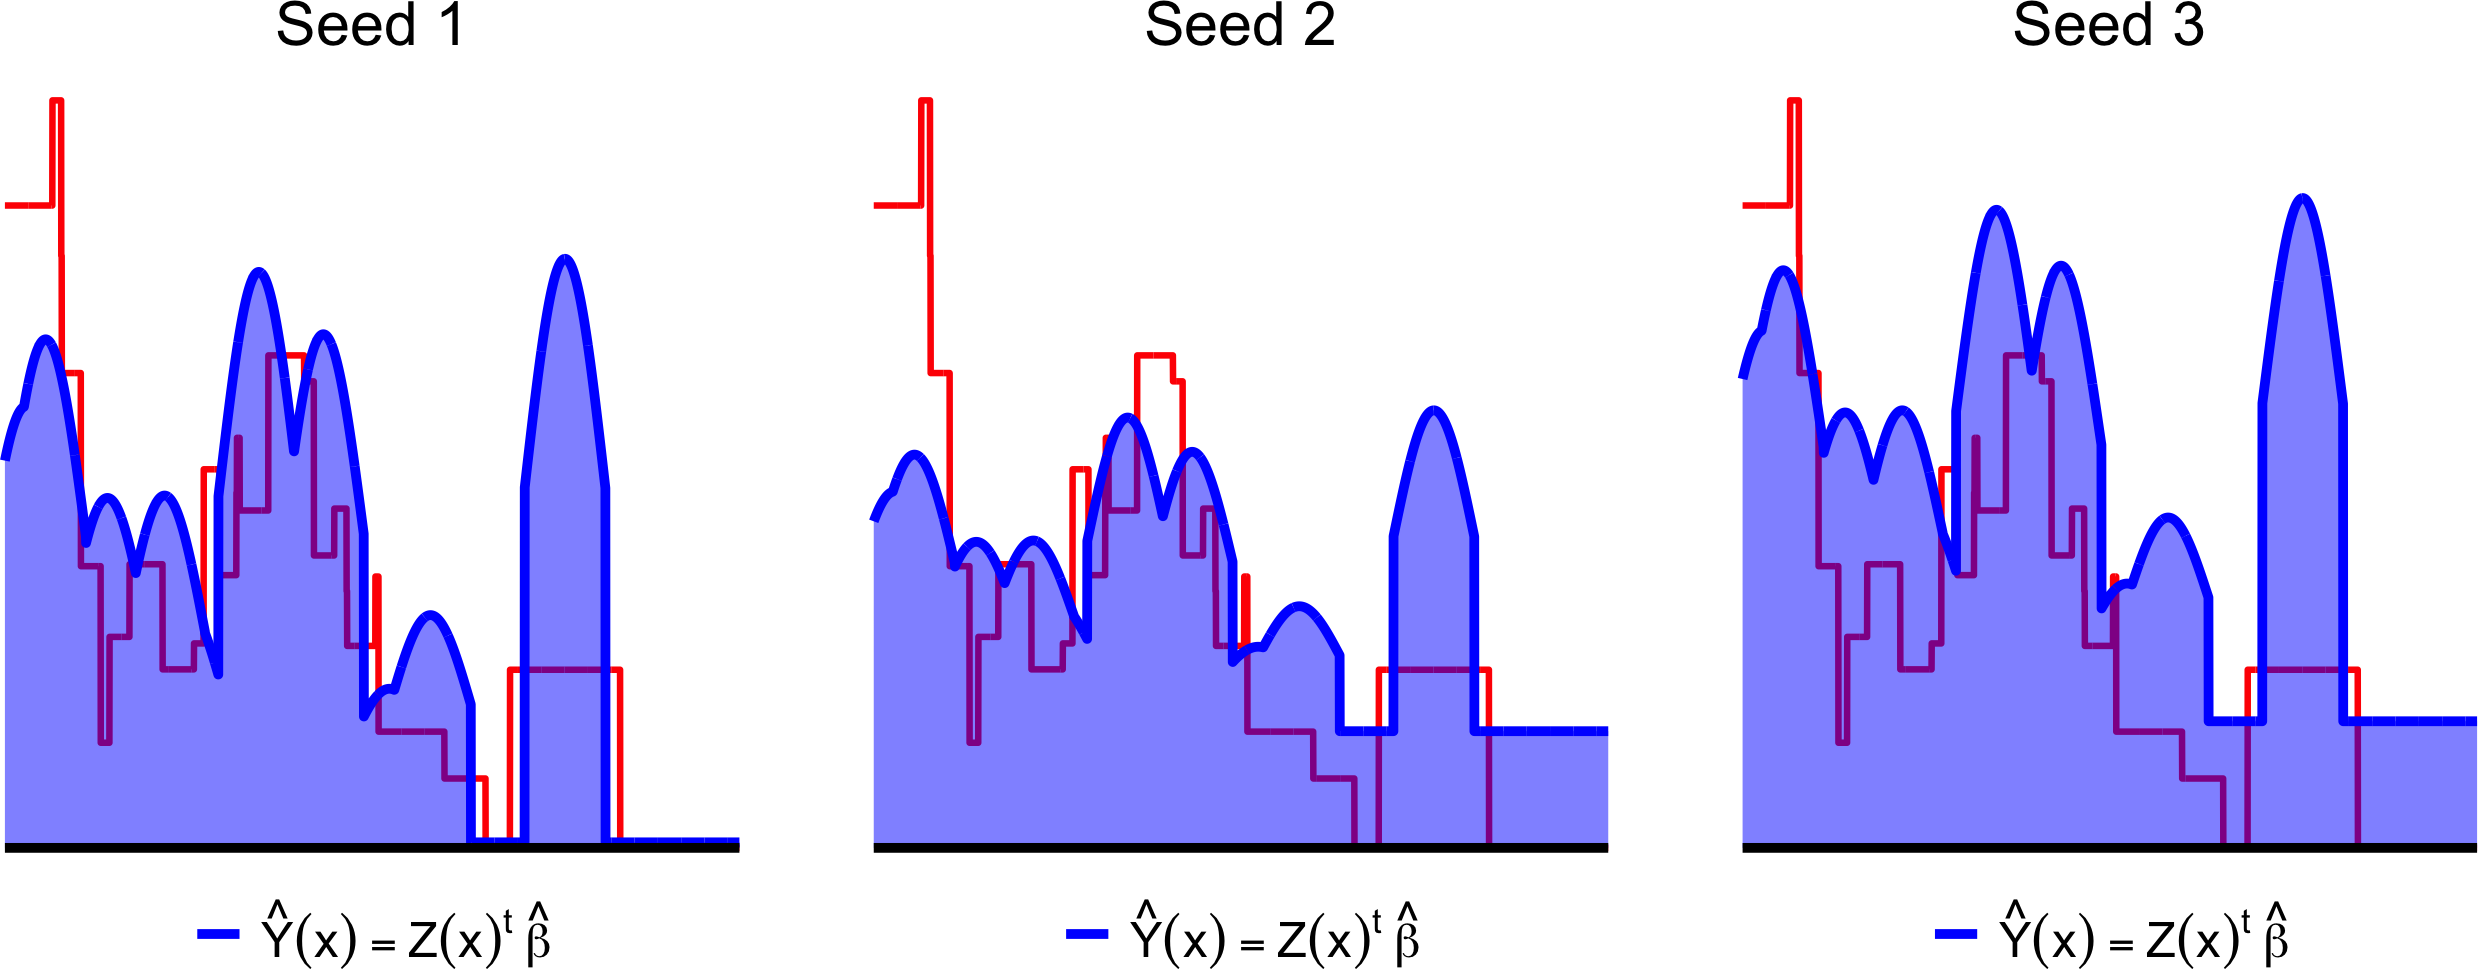
\includegraphics[width=1\linewidth,height=\textheight,keepaspectratio]{monte_carlo_interpretation_beamer_files/figure-beamer/unnamed-chunk-9-1.png}
\end{center}
\end{frame}

\begin{frame}{Close your eyes and treat internal as external\ldots{}}
\phantomsection\label{close-your-eyes-and-treat-internal-as-external}
\begin{block}{The "external model assumption"}
If an \textbf{internal} model (fit using $s$ itself, or data dependent on it) is \textit{treated as if} it were external, we are making the \textbf{external model assumption}.
\end{block}

\begin{itemize}
\setlength{\itemsep}{0.2cm}

\item Only \textbf{asymptotically} design-unbiased results for most reasonable model classes.

\item Asymptotic validity is likely but not automatic --- \textbf{someone has to do the work} to demonstrate it holds for the specific model class being used.

\item See Breidt \& Opsomer, 2017 for demonstration for many modern modeling classes.
\end{itemize}

\pause

\begin{block}{Takeaway}
\textit{External} $\implies$ exact design-unbiasedness, no restrictions on the model. \newline \textit{Internal, assumed external} $\implies$ asymptotic unbiasedness when justified for model-class.
\end{block}
\end{frame}




\end{document}
